\section{Úvod}
Dátové štruktúry a algoritmy tvoria základnú, prvotnú časť výučby 
informatiky. Vizualizácia algoritmov a dátových štruktúr je grafické 
znázornenie, ktoré abstrahuje od implementačných detajlov a reprezentácie
v pamäti. Je teda vhodnou pomôckou pri výučbe i samoštúdiu. 

Ukážka nášho softvéru \emph{Gnarley Trees} je na obrázku~\ref{img:historia}.
Tento projekt začal ako bakalárska práca Jakuba Kováča \citep{kuko};
v tomto článku popisujeme nové dátové štruktúry, ktoré sme vizualizovali
a nové funkcie a vylepšenia, ktoré sme doplnili.

% Ako ľudia so záujmom o dátové štruktúry sme sa rozhodli pomôcť vybudovať 
% dobrý softvér na vizualizáciu algoritmov a dátových štruktúr a obohatiť 
% kompiláciu Jakuba Kováča \citep{kuko} o ďalšie dátové štruktúry. 
Z vyvažovaných stromov vizualizujeme
\emph{B$^+$-strom}, \emph{strom s prstom} a \emph{strom s reverzami}, z háld to sú \emph{d-árna 
halda}, \emph{ľavicová halda}, \emph{skew halda} a \emph{párovacia halda}. 
Taktiež vizualizujeme aj \emph{union-find problém} a 
\emph{písmenkový strom (trie)}. 

Okrem vizualizácie softvér prerábame a neustále vylepšujeme.
Doplnili sme ho o históriu krokov a operácií, jednoduchšie ovládanie
a veľa ďalších funkcií. Softvér je celý v slovenčine aj angličtine a je 
implementovaný v jazyku \texttt{Java}. Dostupný je na stránke
\hbox{\url{http://people.ksp.sk/~kuko/gnarley-trees}} vo forme appletov
s jednotlivými dátovými štruktúrami, a tiež vo forme samostatného programu,
ktorý obsahuje všetky dátové štruktúry a je určený na používanie offline.

Našou snahou je vytvoriť kvalitný softvér nezávislý od operačného systému, 
ktorý bude vyhovovať ako pomôcka pri výučbe ako aj pri samoštúdiu a bude
voľne prístupný. 

%\bigskip
Predchádzajúci výskum v oblasti pedagogiky
zatiaľ nedokázal úplne preukázať pedagogickú efektívnosť
vizualizácií \citep{shaffer}, avšak viacero štúdií potvrdilo zvýšený záujem
a zapojenosť študentov \citep{naps02, hundhausen02}.

Rozmach vizualizácie algoritmov priniesla najmä {\tt Java} a jej fungovanie 
bez viazanosti na konkrétny operačný systém. Kvalita iných existujúcich vizualizácií sa líši 
a keďže ide o ľahko naprogramovateľné programy, je ich veľa a sú pomerne 
nekvalitné \citep{shaffer}. 
Zbieraním a analyzovaním kvality sa venuje skupina AlgoViz (\hbox{\url{http://algoviz.org/}}).

Zaujímavé je pozorovanie, že určovanie si vlastného tempa pri vizualizácií 
je veľká pomôcka. Naopak, ukazovanie pseudokódu alebo nemožnosť určenia si
vlastného tempa (napríklad animácia bez možnosti pozastavenia), takmer 
žiadne zlepšenie neprináša \citep{shaffer,saraiya}.

%\bigskip
Zvyšok článku je organizovaný nasledovne: V sekcií 2 popisujeme implementované
vylepšenia týkajúce sa vizualizácie, grafiky a ovládania, v sekciách 3 až 6
nové dátové štruktúry, ktoré sme implementovali a vizualizovali: vyvážené
stromy, haldy, union-find a písmenkové stromy.

\begin{figure*}
\centering
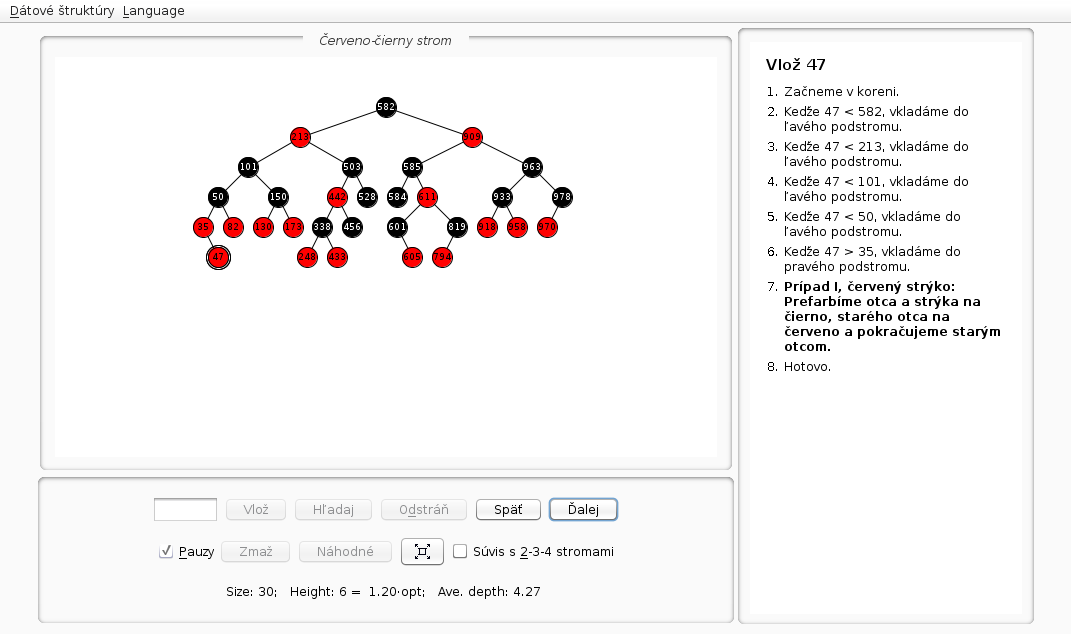
\includegraphics[width=2.01\columnwidth]{obrazky/gt.png}
\caption{\emph{Softvér Gnarley Trees.} V ovládacom paneli dole môže užívateľ
zvoliť operáciu a vstupnú hodnotu a sledovať priebeh algoritmu (monentálne vkladanie
prvku 47). Užívateľ postupuje vlastným tempom  pomocou tlačidiel \uv{Ďalej}, prípadne
\uv{Späť}. Vpravo je popis vykonávaných krokov; kliknutím na konkrétny krok v histórií
sa môže užívateľ vrátiť.}
\label{img:historia} 
\end{figure*}
